\documentclass{article} % For LaTeX2e
\usepackage{amsmath}
\usepackage{amsfonts,dsfont}
\usepackage{amssymb}
\usepackage[ruled,vlined]{algorithm2e}

\usepackage{graphicx}
\usepackage{caption}
\usepackage{subcaption}

\DeclareMathOperator*{\argmin}{arg\,min}
\DeclareMathOperator*{\argmax}{arg\,max}

\begin{document}

\section{Compact Description For Anomalies}

Providing explanations for anomalies is important and some recent work (among others) can be found in \cite{macha:2017}. We illustrate a very simple approach when AAD is used with \textit{Isolation Forest}.

The Isolation Forest version of AAD works by partitioning the space into smaller subspaces and weights each subspace to fit the expert feedback. The end result is: (1) a set of default (unsupervised) anomaly scores for each subspace and, (2) weights for each subspace inferred from feedback. We can generate compact descriptions for the anomalies using this information. The idea is to select some combination of (preferably) the smallest subspaces that \textbf{cover} all \textbf{discovered} anomalies. Therefore, we treat this as an instance of the \emph{set covering} problem. We illustrate this on a toy dataset below.

Assume that there are total $m$ subspaces across all Isolation Forest trees. We represent weights by ${\bf w} \in \mathbb{R}^m$, and the corresponding unsupervised anomaly scores by ${\bf d} \in \mathbb{R}^m$.

Now, the final anomaly scores for the \textbf{subspaces} (not instances), after incorporating feedback, is ${\bf a} = {\bf w} \circ {\bf d} \in \mathbb{R}^m$ where $\circ$ denotes the element wise (\textit{Hadamard}) product.

We sort the scores in ${\bf a}$ in descending order and select (say) $30$ top ranked subspaces. Next, we retain only those subspaces from this set which contain at least one anomaly \textbf{discovered} by the analyst. Let us denote the resulting set of subspaces by $\mathcal{S}$. Further, let $\mathcal{Z}$ be the set of discovered anomalies that belong to one or more subspaces in $\mathcal{S}$, and $|\mathcal{Z}|=n$. (Note that some of the discovered anomalies might not belong to any of the top ranked subspaces we selected.)

Let $|\mathcal{S}|=k$. Denote the \textit{volumes} of the subspaces in $\mathcal{S}$ by the vector ${\bf v} \in \mathbb{R}^k$. Now, assume that a binary vector ${\bf x} \in \{0, 1\}^k$ contains $1$ in locations corresponding to the subspaces in $\mathcal{S}$ which are included in the covering set, and $0$ otherwise. Let ${\bf u}_z \in \{0, 1\}^k$ denote a vector for each anomaly $z \in \mathcal{Z}$ which contains $1$ in all locations corresponding to the subspaces in $\mathcal{S}$ that $z$ belongs to. Let ${\bf U} \in \{0, 1\}^{[n \times k]}$ represent the matrix of all ${\bf u}$s.

The selection of the compact set of subspaces to describe all discovered anomalies can be formulated as:
\begin{align}
& \argmin_{{\bf x} \in \{0, 1\}^k} {\bf x} \cdot {\bf v}^p \label{eqn:opt} \\
\text{s.t.} & {\bf U} \cdot {\bf x} \geq {\bf 1} \nonumber \\
\text{where, } & \text{${\bf 1}$ is the column vector of $n$ 1s, and} \nonumber \\
& \text{$p$ is an integer $\geq 1$ (more below)} \nonumber
\end{align}

The parameter $p$ determines how severely to penalize larger volumes. This is usually $1$. However, a larger value will strongly discourage bigger volume subspaces from being selected.

Note that we have not considered labeled nominals in the optimization objective, but a more sophisticated objective might include them too.

We apply this idea on a toy data shown in Figure~\ref{fig:dataset}. The compact descriptions are shown in Figure~\ref{fig:compact_rects}.

\begin{figure}
	\centering
	\begin{subfigure}[b]{0.3\textwidth}
		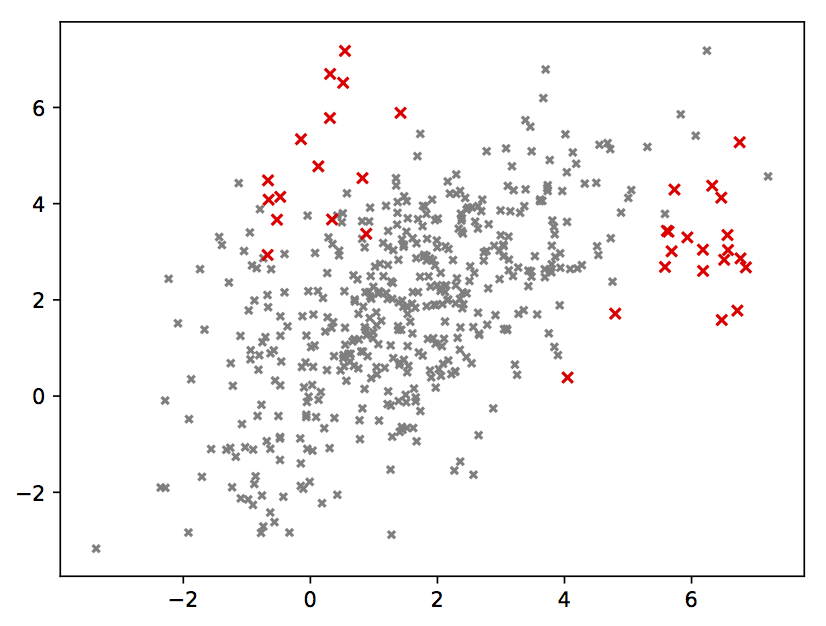
\includegraphics[width=\textwidth]{toy2_dataset}
		\caption{Dataset}
		\label{fig:dataset}
	\end{subfigure}
	~ %add desired spacing between images, e. g. ~, \quad, \qquad, \hfill etc. 
	%(or a blank line to force the subfigure onto a new line)
	\begin{subfigure}[b]{0.3\textwidth}
		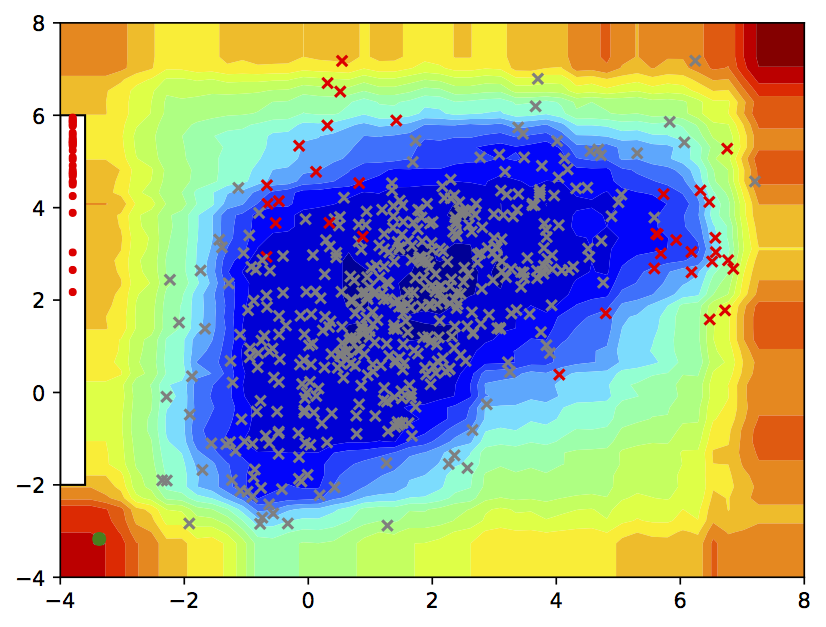
\includegraphics[width=\textwidth]{toy2_iter_00}
		\caption{Initial score contours}
		\label{fig:baseline_contours}
	\end{subfigure}
	~ %add desired spacing between images, e. g. ~, \quad, \qquad, \hfill etc. 
	%(or a blank line to force the subfigure onto a new line)
	\begin{subfigure}[b]{0.3\textwidth}
		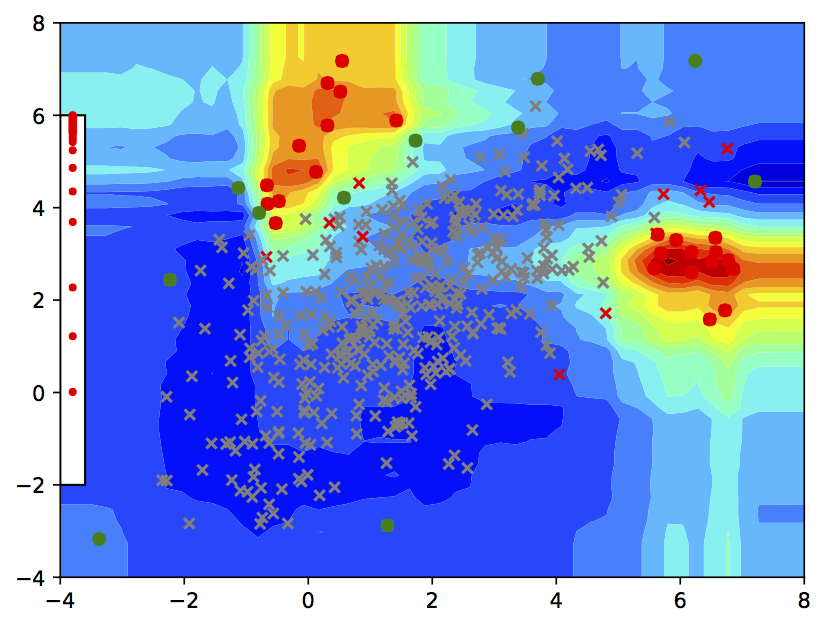
\includegraphics[width=\textwidth]{toy2_iter_34}
		\caption{After 35 feedback}
		\label{fig:contours_35}
	\end{subfigure}
	\caption{Dataset and score contours. Figure~\ref{fig:dataset} shows a synthetic toy dataset. Figure~\ref{fig:baseline_contours} shows the initial Isolation Forest score contours. Figure~\ref{fig:contours_35} shows the score contours after 35 feedback iterations from the Oracle. The red dots are discovered anomalies (true positives). The green dots are discovered nominals (false positives). The red checks are undiscovered anomalies (false negatives).} \label{fig:dataset_and_contours}
\end{figure}

\begin{figure}
	\centering
	\begin{subfigure}[b]{0.3\textwidth}
		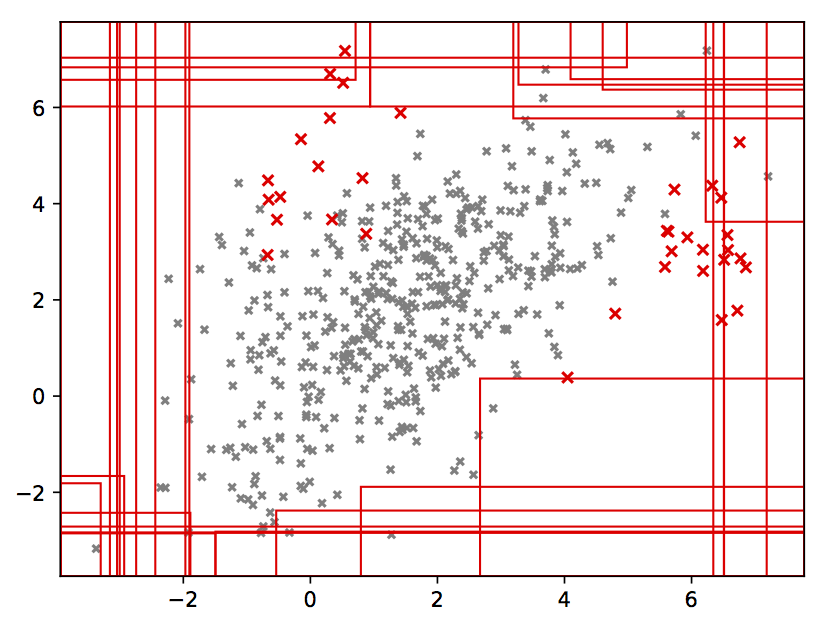
\includegraphics[width=\textwidth]{top_30_anomalous_regions_100_trees_baseline}
		\caption{Baseline}
		\label{fig:baseline_rects}
	\end{subfigure}
	~ %add desired spacing between images, e. g. ~, \quad, \qquad, \hfill etc. 
	%(or a blank line to force the subfigure onto a new line)
	\begin{subfigure}[b]{0.3\textwidth}
		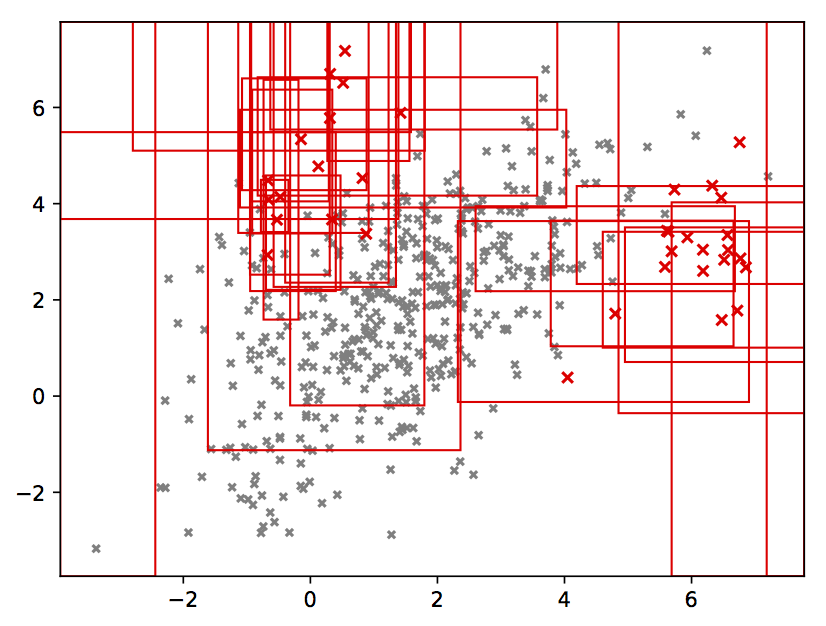
\includegraphics[width=\textwidth]{top_30_anomalous_regions_100_trees_aad}
		\caption{AAD}
		\label{fig:aad_rects}
	\end{subfigure}
	~ %add desired spacing between images, e. g. ~, \quad, \qquad, \hfill etc. 
	%(or a blank line to force the subfigure onto a new line)
	\begin{subfigure}[b]{0.3\textwidth}
		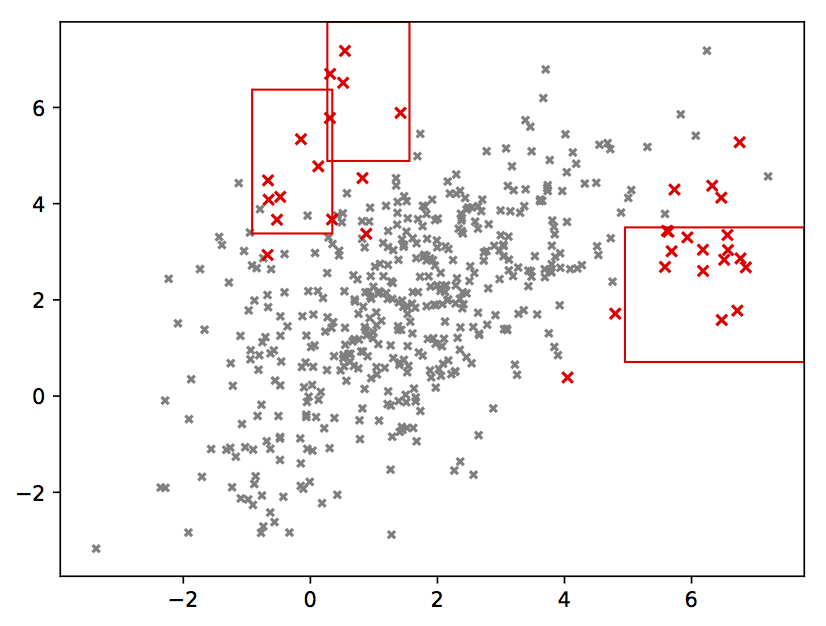
\includegraphics[width=\textwidth]{top_30_anomalous_regions_100_trees_compact}
		\caption{Compact AAD}
		\label{fig:compact_rects}
	\end{subfigure}
	\caption{Top $30$ subspaces ranked by ${\bf w}\circ{\bf d}$. Figure~\ref{fig:baseline_rects} shows the top $30$ subspaces with no feedback. We can see that most of these are just the exterior regions of the dataset. Figure~\ref{fig:aad_rects} shows that after feedback, the most anomalous subspaces are those around the labeled anomalies. Figure~\ref{fig:compact_rects} shows the most compact set of subspaces (for AAD) which cover all labeled anomalies. These are computed with Equation~\ref{eqn:opt}. Note that the compact subspaces only cover anomalies that were discovered in the $35$ feedback iterations. Anomalies which were not detected are likely to fall outside these compact subspaces.} \label{fig:rects}
\end{figure}

\begin{thebibliography}{1}
\bibitem{macha:2017} Meghanath Macha and Leman Akoglu {\em {X-PACS:} eXPlaining Anomalies by Characterizing Subspaces},  2017, http://arxiv.org/abs/1708.05929.
\end{thebibliography}

\end{document}
